\documentclass[a4paper,12pt]{article}
\usepackage{xcolor}
\usepackage{amsmath,amsfonts,amssymb}
\usepackage{geometry}
\usepackage{fancyhdr}
\usepackage{graphicx}
\usepackage{subcaption} % For subfigure support
\usepackage{float} % For [H] placement
\usepackage{titlesec}
\usepackage{tikz}
\usepackage{booktabs}
\usepackage{array}
\usetikzlibrary{shadows}
\usepackage{tcolorbox}
\usepackage{float}
\usepackage{lipsum}
\usepackage{mdframed}
\usepackage{pagecolor}
\usepackage{mathpazo}   % Palatino font (serif)
\usepackage{microtype}  % Better typography

% Page background color
\pagecolor{gray!10!white}

% Geometry settings
\geometry{margin=0.5in}
\pagestyle{fancy}
\fancyhf{}

% Fancy header and footer
\fancyhead[C]{\textbf{\color{blue!80}CS754 Assignment-1}}
% \fancyhead[R]{\color{blue!80}Saksham Rathi}
\fancyfoot[C]{\thepage}

% Custom Section Color and Format with Sans-serif font
\titleformat{\section}
{\sffamily\color{purple!90!black}\normalfont\Large\bfseries}
{\thesection}{1em}{}

% Custom subsection format
\titleformat{\subsection}
{\sffamily\color{cyan!80!black}\normalfont\large\bfseries}
{\thesubsection}{1em}{}

% Stylish Title with TikZ (Enhanced with gradient)
\newcommand{\cooltitle}[1]{%
  \begin{tikzpicture}
    \node[fill=blue!20,rounded corners=10pt,inner sep=12pt, drop shadow, top color=blue!50, bottom color=blue!30] (box)
    {\Huge \bfseries \color{black} #1};
  \end{tikzpicture}
}
\usepackage{float} % Add this package

\newenvironment{solution}[2][]{%
    \begin{mdframed}[linecolor=blue!70!black, linewidth=2pt, roundcorner=10pt, backgroundcolor=yellow!10!white, skipabove=12pt, skipbelow=12pt]%
        \textbf{\large #2}
        \par\noindent\rule{\textwidth}{0.4pt}
}{
    \end{mdframed}
}

% Document title
\title{\cooltitle{CS754 Assignment-1}}
\author{{\bf Saksham Rathi, Ekansh Ravi Shankar, Kshitij Vaidya}}
\date{}

\begin{document}
\maketitle

\textbf{Declaration:} The work submitted is our own, and we have adhered to the principles of academic honesty while completing and submitting this work. We have not referred to any unauthorized sources, and we have not used generative AI tools for the work submitted here.

\section*{Question 5}

\begin{solution}{OMP}
The code is present in the file \texttt{assignment1/5/code/omp.m}. On opening matlab in that folder, the code can be run by executing the command \texttt{omp}.

Firstly, we need to plot RMSE vs m (number of measurements), for various values of sparsity $k$. 

\begin{figure}[H]
  \centering
  % First subfigure
  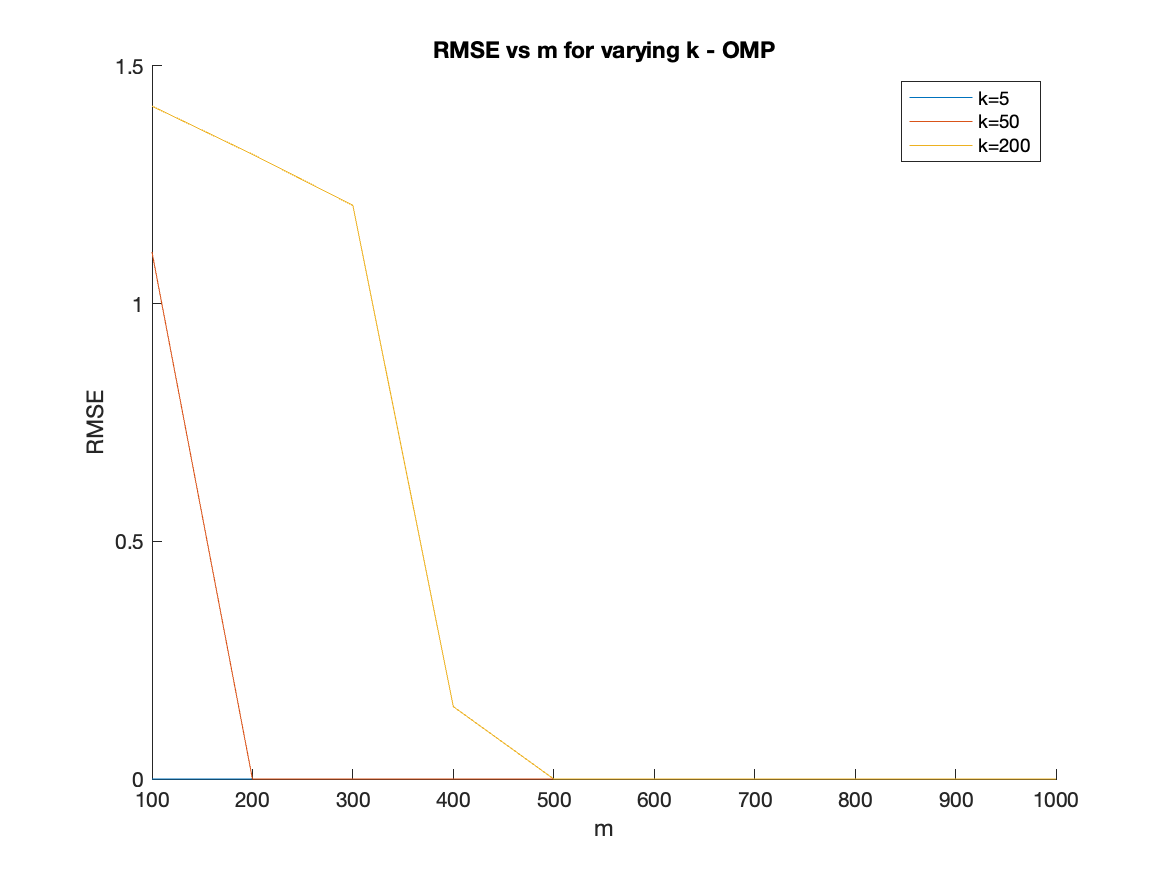
\includegraphics[width=0.5\textwidth]{../images/omp/omp_k.png}
  \caption{Comparison of RMSE vs m for different values of $k$ for OMP}
  \label{fig:rmse_comparison}
\end{figure}

From the above plot, we can see that OMP performs really well, because RMSE is very low for almost all values of $m$. It decreases as $m$ increases, which is expected as more measurements should lead to better reconstruction. The RMSE is lower for higher various values of $k$ (sparsity level), which is again as expected as higher sparsity level should make reconstruction easier.


Next, we plot RMSE vs $k$ for various values of $m$.

\begin{figure}[H]
  \centering
  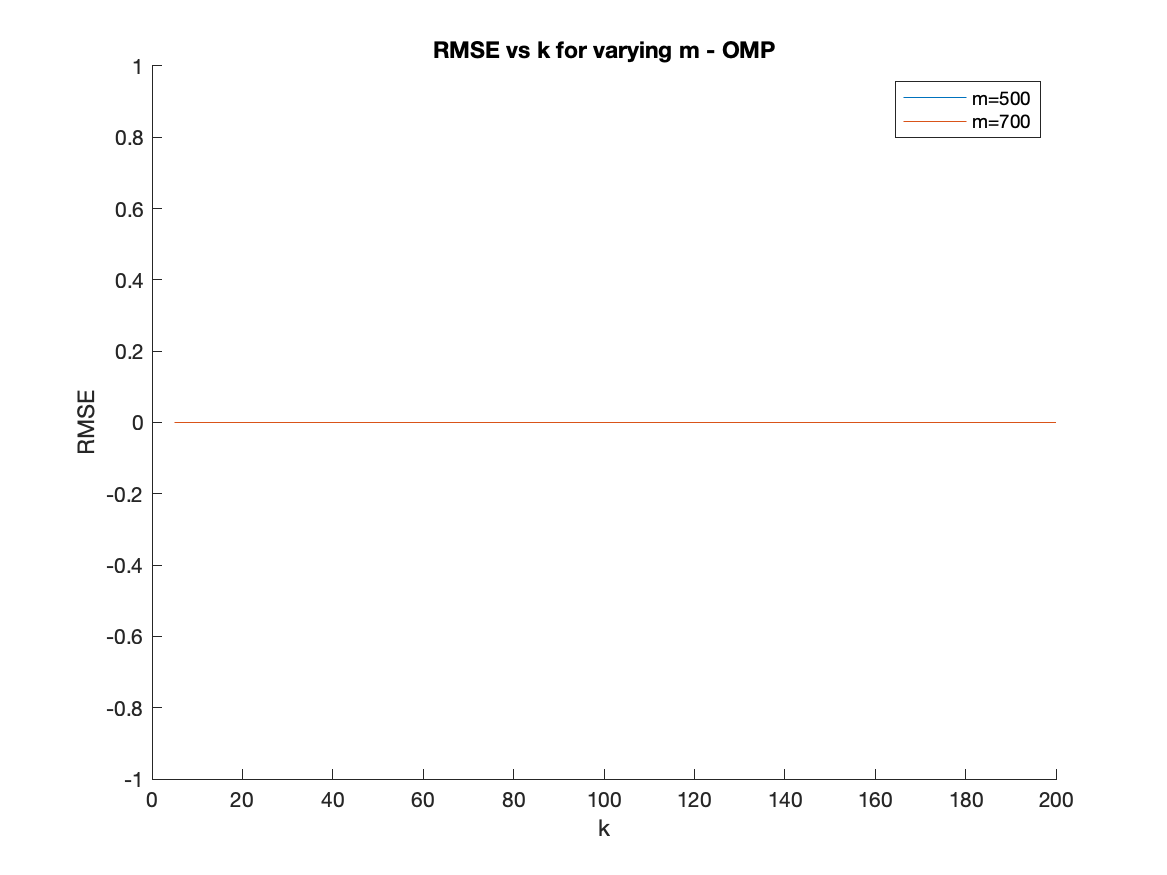
\includegraphics[width=0.5\textwidth]{../images/omp/omp_m.png}
  \caption{Comparison of RMSE vs k for different values of $m$ for OMP}
  \label{fig:rmse_comparison2}
\end{figure}


In general, as $k$ increases (increase in the number of non-zero indices), the RMSE increases. This is expected, as a higher sparsity level makes reconstruction harder. Some fluctuations in the RMSE for intermediate values of $k$ could be due to the randomness in the measurement matrix or noise in the reconstruction.

Here is the ground truth images for various values of $k$:

\begin{figure}[H]
  \centering
  \begin{subfigure}[t]{0.32\textwidth}
      \centering
      
\includegraphics[width=\textwidth]{../images/omp/Ground_Truth_k_5.png}
      \caption{Ground truth for $k = 5$}
  \end{subfigure}
  \begin{subfigure}[t]{0.32\textwidth}
      \centering
      \includegraphics[width=\textwidth]{../images/omp/Ground_truth_k_50.png}
      \caption{Ground truth for $k = 50$}
  \end{subfigure}
  \begin{subfigure}[t]{0.32\textwidth}
      \centering
      \includegraphics[width=\textwidth]{../images/omp/Ground_truth_k_200.png}
      \caption{Ground truth for $k = 200$}
  \end{subfigure}
  \caption{Ground truth images for different values of $k$}
  \label{fig:ground_truth}
\end{figure}

Here are the corresponding reconstructed images for various $m$ values \texttt{images/omp} folder:

\begin{figure}[H]
  \centering
  % First row
  \begin{subfigure}[t]{0.23\textwidth}
      \centering
      
\includegraphics[width=\textwidth]{../images/omp/Reconstructed_k_5_m_100.png}
      \caption{Reconstructed for $k = 5$, $m = 100$}
  \end{subfigure}
    \begin{subfigure}[t]{0.23\textwidth}
        \centering
        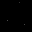
\includegraphics[width=\textwidth]{../images/omp/Reconstructed_k_5_m_200.png}
        \caption{Reconstructed for $k = 5$, $m = 200$}
    \end{subfigure}
    \begin{subfigure}[t]{0.23\textwidth}
        \centering
        
\includegraphics[width=\textwidth]{../images/omp/Reconstructed_k_5_m_300.png}
        \caption{Reconstructed for $k = 5$, $m = 300$}
    \end{subfigure}
    \begin{subfigure}[t]{0.23\textwidth}
        \centering
        
\includegraphics[width=\textwidth]{../images/omp/Reconstructed_k_5_m_400.png}
        \caption{Reconstructed for $k = 5$, $m = 400$}
    \end{subfigure}\\
    \begin{subfigure}[t]{0.23\textwidth}
        \centering
        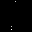
\includegraphics[width=\textwidth]{../images/omp/Reconstructed_k_5_m_500.png}
        \caption{Reconstructed for $k = 5$, $m = 500$}
    \end{subfigure}
    \begin{subfigure}[t]{0.23\textwidth}
        \centering
        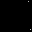
\includegraphics[width=\textwidth]{../images/omp/Reconstructed_k_5_m_600.png}
        \caption{Reconstructed for $k = 5$, $m = 600$}
    \end{subfigure}
    \begin{subfigure}[t]{0.23\textwidth}
        \centering
        
\includegraphics[width=\textwidth]{../images/omp/Reconstructed_k_5_m_700.png}
        \caption{Reconstructed for $k = 5$, $m = 700$}
    \end{subfigure}
    \begin{subfigure}[t]{0.23\textwidth}
        \centering
        
\includegraphics[width=\textwidth]{../images/omp/Reconstructed_k_5_m_800.png}
        \caption{Reconstructed for $k = 5$, $m = 800$}
    \end{subfigure}\\
    \begin{subfigure}[t]{0.23\textwidth}
        \centering
        
\includegraphics[width=\textwidth]{../images/omp/Reconstructed_k_5_m_900.png}
        \caption{Reconstructed for $k = 5$, $m = 900$}
    \end{subfigure}
    \begin{subfigure}[t]{0.23\textwidth}
        \centering
        
\includegraphics[width=\textwidth]{../images/omp/Reconstructed_k_5_m_1000.png}
        \caption{Reconstructed for $k = 5$, $m = 1000$}
    \end{subfigure}
    \begin{subfigure}[t]{0.23\textwidth}
        \centering
        
\includegraphics[width=\textwidth]{../images/omp/Reconstructed_k_50_m_100.png}
        \caption{Reconstructed for $k = 50$, $m = 100$}
    \end{subfigure}
    \begin{subfigure}[t]{0.23\textwidth}
        \centering
        
\includegraphics[width=\textwidth]{../images/omp/Reconstructed_k_50_m_200.png}
        \caption{Reconstructed for $k = 50$, $m = 200$}
    \end{subfigure}\\
    \begin{subfigure}[t]{0.23\textwidth}
        \centering
        
\includegraphics[width=\textwidth]{../images/omp/Reconstructed_k_50_m_300.png}
        \caption{Reconstructed for $k = 50$, $m = 300$}
    \end{subfigure}
    \begin{subfigure}[t]{0.23\textwidth}
        \centering
        
\includegraphics[width=\textwidth]{../images/omp/Reconstructed_k_50_m_400.png}
        \caption{Reconstructed for $k = 50$, $m = 400$}
    \end{subfigure}
    \begin{subfigure}[t]{0.23\textwidth}
        \centering
        
\includegraphics[width=\textwidth]{../images/omp/Reconstructed_k_50_m_500.png}
        \caption{Reconstructed for $k = 50$, $m = 500$}
    \end{subfigure}
    \begin{subfigure}[t]{0.23\textwidth}
        \centering
        
\includegraphics[width=\textwidth]{../images/omp/Reconstructed_k_50_m_600.png}
        \caption{Reconstructed for $k = 50$, $m = 600$}
    \end{subfigure}\\
    \begin{subfigure}[t]{0.23\textwidth}
        \centering
        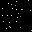
\includegraphics[width=\textwidth]{../images/omp/Reconstructed_k_50_m_700.png}
        \caption{Reconstructed for $k = 50$, $m = 700$}
    \end{subfigure}
    \begin{subfigure}[t]{0.23\textwidth}
        \centering
        
\includegraphics[width=\textwidth]{../images/omp/Reconstructed_k_50_m_800.png}
        \caption{Reconstructed for $k = 50$, $m = 800$}
    \end{subfigure}
    \begin{subfigure}[t]{0.23\textwidth}
        \centering
        
\includegraphics[width=\textwidth]{../images/omp/Reconstructed_k_50_m_900.png}
        \caption{Reconstructed for $k = 50$, $m = 900$}
    \end{subfigure}
    \begin{subfigure}[t]{0.23\textwidth}
        \centering
        
\includegraphics[width=\textwidth]{../images/omp/Reconstructed_k_50_m_1000.png}
        \caption{Reconstructed for $k = 50$, $m = 1000$}
    \end{subfigure}
  \caption{Reconstructed images for different values of $k$ and $m$}
  \label{fig:reconstructed_all}
\end{figure}

\begin{figure}[H]
    \centering
  % First row
  \begin{subfigure}[t]{0.23\textwidth}
      \centering
      
\includegraphics[width=\textwidth]{../images/omp/Reconstructed_k_200_m_100.png}
      \caption{Reconstructed for $k = 200$, $m = 100$}
  \end{subfigure}
    \begin{subfigure}[t]{0.23\textwidth}
        \centering
        
\includegraphics[width=\textwidth]{../images/omp/Reconstructed_k_200_m_200.png}
        \caption{Reconstructed for $k = 200$, $m = 200$}
    \end{subfigure}
    \begin{subfigure}[t]{0.23\textwidth}
        \centering
        
\includegraphics[width=\textwidth]{../images/omp/Reconstructed_k_200_m_300.png}
        \caption{Reconstructed for $k = 200$, $m = 300$}
    \end{subfigure}
    \begin{subfigure}[t]{0.23\textwidth}
        \centering
        
\includegraphics[width=\textwidth]{../images/omp/Reconstructed_k_200_m_400.png}
        \caption{Reconstructed for $k = 200$, $m = 400$}
    \end{subfigure}\\
    \begin{subfigure}[t]{0.23\textwidth}
        \centering
        
\includegraphics[width=\textwidth]{../images/omp/Reconstructed_k_200_m_500.png}
        \caption{Reconstructed for $k = 200$, $m = 500$}
    \end{subfigure}
    \begin{subfigure}[t]{0.23\textwidth}
        \centering
        
\includegraphics[width=\textwidth]{../images/omp/Reconstructed_k_200_m_600.png}
        \caption{Reconstructed for $k = 200$, $m = 600$}
    \end{subfigure}
    \begin{subfigure}[t]{0.23\textwidth}
        \centering
        
\includegraphics[width=\textwidth]{../images/omp/Reconstructed_k_200_m_700.png}
        \caption{Reconstructed for $k = 200$, $m = 700$}
    \end{subfigure}
    \begin{subfigure}[t]{0.23\textwidth}
        \centering
        
\includegraphics[width=\textwidth]{../images/omp/Reconstructed_k_200_m_800.png}
        \caption{Reconstructed for $k = 200$, $m = 800$}
    \end{subfigure}\\
    \begin{subfigure}[t]{0.23\textwidth}
        \centering
        
\includegraphics[width=\textwidth]{../images/omp/Reconstructed_k_200_m_900.png}
        \caption{Reconstructed for $k = 200$, $m = 900$}
    \end{subfigure}
    \begin{subfigure}[t]{0.23\textwidth}
        \centering
        
\includegraphics[width=\textwidth]{../images/omp/Reconstructed_k_200_m_1000.png}
        \caption{Reconstructed for $k = 200$, $m = 1000$}
    \end{subfigure}
    \caption{Reconstructed images for different values of $k$ and $m$}
    \label{fig:reconstructed_all2}
\end{figure}
\end{solution}

\begin{solution}{COSAMP}
    The code is present in the file \texttt{assignment1/5/code/cosamp.m}. On opening matlab in that folder, the code can be run by executing the command \texttt{cosamp}.
    
    Firstly, we need to plot RMSE vs m (number of measurements), for various values of sparsity $k$. 
    
    \begin{figure}[H]
      \centering
      % First subfigure
      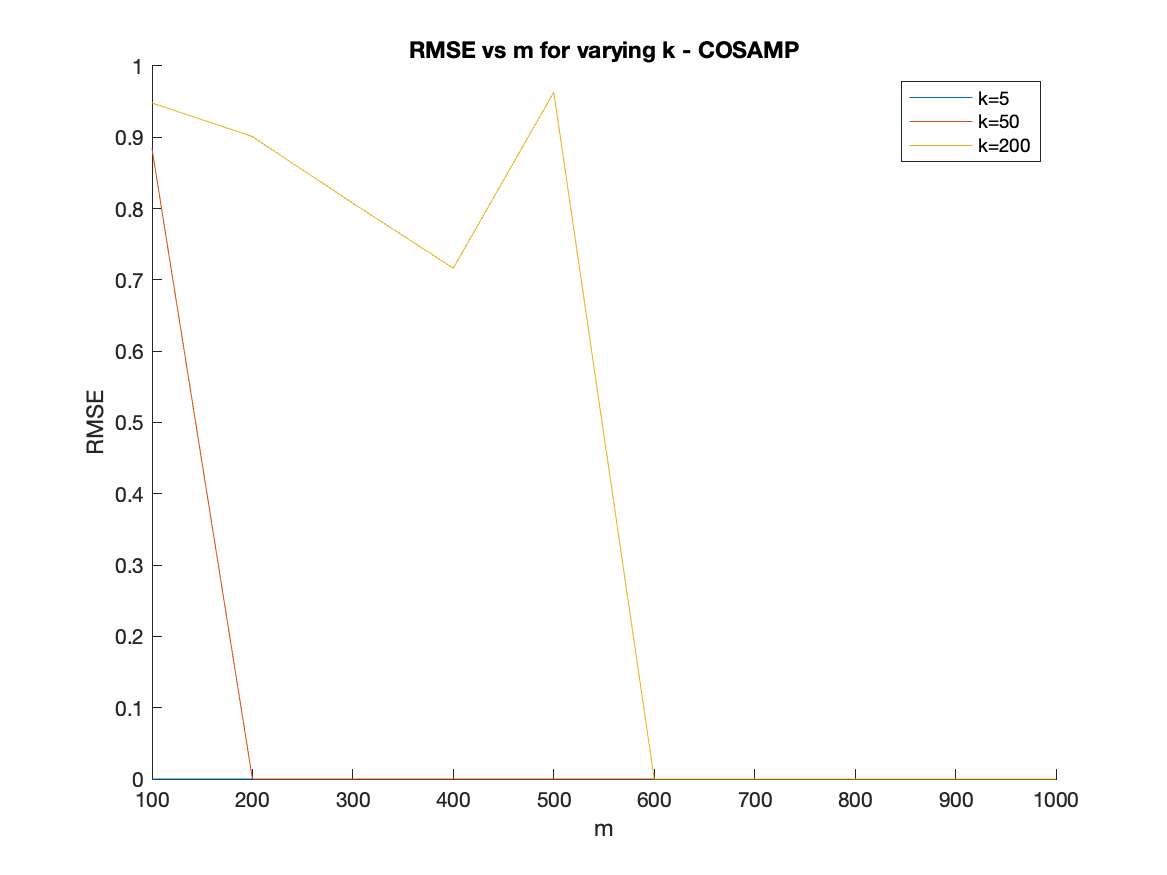
\includegraphics[width=0.5\textwidth]{../images/cosamp/cosamp_k.png}
      \caption{Comparison of RMSE vs m for different values of $k$ for COSAMP}
      \label{fig:rmse_comparison}
    \end{figure}
    
    From the above plot, we can see that COSAMP performs really well (although not as good as OMP for some values of $m$). It decreases as $m$ increases, which is expected as more measurements should lead to better reconstruction. The RMSE is lower for higher various values of $k$ (sparsity level), which is again as expected as higher sparsity level should make reconstruction easier.
    
    
    Next, we plot RMSE vs $k$ for various values of $m$.
    
    \begin{figure}[H]
      \centering
      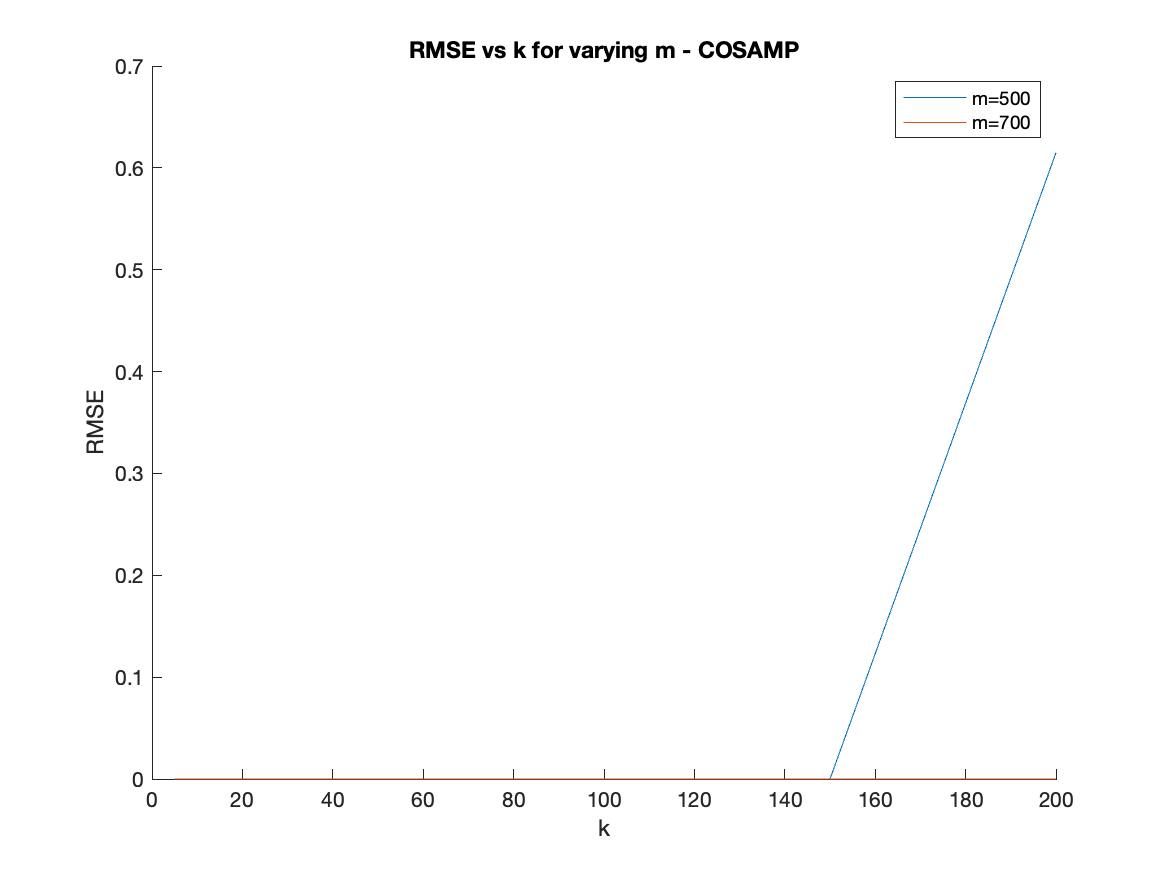
\includegraphics[width=0.5\textwidth]{../images/cosamp/cosamp_m.png}
      \caption{Comparison of RMSE vs k for different values of $m$ for cosamp}
      \label{fig:rmse_comparison2}
    \end{figure}
    
    
    In general, as $k$ increases (increase in the number of non-zero indices), the RMSE increases. This is expected, as a higher sparsity level makes reconstruction harder.
    
    Here is the ground truth images for various values of $k$:
    
    \begin{figure}[H]
      \centering
      \begin{subfigure}[t]{0.32\textwidth}
          \centering
          
\includegraphics[width=\textwidth]{../images/cosamp/Ground_Truth_k_5.png}
          \caption{Ground truth for $k = 5$}
      \end{subfigure}
      \begin{subfigure}[t]{0.32\textwidth}
          \centering
          \includegraphics[width=\textwidth]{../images/cosamp/Ground_truth_k_50.png}
          \caption{Ground truth for $k = 50$}
      \end{subfigure}
      \begin{subfigure}[t]{0.32\textwidth}
          \centering
          \includegraphics[width=\textwidth]{../images/cosamp/Ground_truth_k_200.png}
          \caption{Ground truth for $k = 200$}
      \end{subfigure}
      \caption{Ground truth images for different values of $k$}
      \label{fig:ground_truth}
    \end{figure}
    
    Here are the corresponding reconstructed images for various $m$ values \texttt{images/cosamp} folder:
    
    \begin{figure}[H]
      \centering
      % First row
      \begin{subfigure}[t]{0.23\textwidth}
          \centering
          
\includegraphics[width=\textwidth]{../images/cosamp/Reconstructed_k_5_m_100.png}
          \caption{Reconstructed for $k = 5$, $m = 100$}
      \end{subfigure}
        \begin{subfigure}[t]{0.23\textwidth}
            \centering
            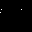
\includegraphics[width=\textwidth]{../images/cosamp/Reconstructed_k_5_m_200.png}
            \caption{Reconstructed for $k = 5$, $m = 200$}
        \end{subfigure}
        \begin{subfigure}[t]{0.23\textwidth}
            \centering
            
\includegraphics[width=\textwidth]{../images/cosamp/Reconstructed_k_5_m_300.png}
            \caption{Reconstructed for $k = 5$, $m = 300$}
        \end{subfigure}
        \begin{subfigure}[t]{0.23\textwidth}
            \centering
            
\includegraphics[width=\textwidth]{../images/cosamp/Reconstructed_k_5_m_400.png}
            \caption{Reconstructed for $k = 5$, $m = 400$}
        \end{subfigure}\\
        \begin{subfigure}[t]{0.23\textwidth}
            \centering
            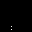
\includegraphics[width=\textwidth]{../images/cosamp/Reconstructed_k_5_m_500.png}
            \caption{Reconstructed for $k = 5$, $m = 500$}
        \end{subfigure}
        \begin{subfigure}[t]{0.23\textwidth}
            \centering
            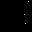
\includegraphics[width=\textwidth]{../images/cosamp/Reconstructed_k_5_m_600.png}
            \caption{Reconstructed for $k = 5$, $m = 600$}
        \end{subfigure}
        \begin{subfigure}[t]{0.23\textwidth}
            \centering
            
\includegraphics[width=\textwidth]{../images/cosamp/Reconstructed_k_5_m_700.png}
            \caption{Reconstructed for $k = 5$, $m = 700$}
        \end{subfigure}
        \begin{subfigure}[t]{0.23\textwidth}
            \centering
            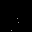
\includegraphics[width=\textwidth]{../images/cosamp/Reconstructed_k_5_m_800.png}
            \caption{Reconstructed for $k = 5$, $m = 800$}
        \end{subfigure}\\
        \begin{subfigure}[t]{0.23\textwidth}
            \centering
            
\includegraphics[width=\textwidth]{../images/cosamp/Reconstructed_k_5_m_900.png}
            \caption{Reconstructed for $k = 5$, $m = 900$}
        \end{subfigure}
        \begin{subfigure}[t]{0.23\textwidth}
            \centering
            
\includegraphics[width=\textwidth]{../images/cosamp/Reconstructed_k_5_m_1000.png}
            \caption{Reconstructed for $k = 5$, $m = 1000$}
        \end{subfigure}
        \begin{subfigure}[t]{0.23\textwidth}
            \centering
            \includegraphics[width=\textwidth]{../images/cosamp/Reconstructed_k_50_m_100.png}
            \caption{Reconstructed for $k = 50$, $m = 100$}
        \end{subfigure}
        \begin{subfigure}[t]{0.23\textwidth}
            \centering
            \includegraphics[width=\textwidth]{../images/cosamp/Reconstructed_k_50_m_200.png}
            \caption{Reconstructed for $k = 50$, $m = 200$}
        \end{subfigure}\\
        \begin{subfigure}[t]{0.23\textwidth}
            \centering
            \includegraphics[width=\textwidth]{../images/cosamp/Reconstructed_k_50_m_300.png}
            \caption{Reconstructed for $k = 50$, $m = 300$}
        \end{subfigure}
        \begin{subfigure}[t]{0.23\textwidth}
            \centering
            \includegraphics[width=\textwidth]{../images/cosamp/Reconstructed_k_50_m_400.png}
            \caption{Reconstructed for $k = 50$, $m = 400$}
        \end{subfigure}
        \begin{subfigure}[t]{0.23\textwidth}
            \centering
            \includegraphics[width=\textwidth]{../images/cosamp/Reconstructed_k_50_m_500.png}
            \caption{Reconstructed for $k = 50$, $m = 500$}
        \end{subfigure}
        \begin{subfigure}[t]{0.23\textwidth}
            \centering
            \includegraphics[width=\textwidth]{../images/cosamp/Reconstructed_k_50_m_600.png}
            \caption{Reconstructed for $k = 50$, $m = 600$}
        \end{subfigure}\\
        \begin{subfigure}[t]{0.23\textwidth}
            \centering
            \includegraphics[width=\textwidth]{../images/cosamp/Reconstructed_k_50_m_700.png}
            \caption{Reconstructed for $k = 50$, $m = 700$}
        \end{subfigure}
        \begin{subfigure}[t]{0.23\textwidth}
            \centering
            \includegraphics[width=\textwidth]{../images/cosamp/Reconstructed_k_50_m_800.png}
            \caption{Reconstructed for $k = 50$, $m = 800$}
        \end{subfigure}
        \begin{subfigure}[t]{0.23\textwidth}
            \centering
            \includegraphics[width=\textwidth]{../images/cosamp/Reconstructed_k_50_m_900.png}
            \caption{Reconstructed for $k = 50$, $m = 900$}
        \end{subfigure}
        \begin{subfigure}[t]{0.23\textwidth}
            \centering
            \includegraphics[width=\textwidth]{../images/cosamp/Reconstructed_k_50_m_1000.png}
            \caption{Reconstructed for $k = 50$, $m = 1000$}
        \end{subfigure}
      \caption{Reconstructed images for different values of $k$ and $m$}
      \label{fig:reconstructed_all}
    \end{figure}
    
    \begin{figure}[H]
        \centering
      % First row
      \begin{subfigure}[t]{0.23\textwidth}
          \centering
          \includegraphics[width=\textwidth]{../images/cosamp/Reconstructed_k_200_m_100.png}
          \caption{Reconstructed for $k = 200$, $m = 100$}
      \end{subfigure}
        \begin{subfigure}[t]{0.23\textwidth}
            \centering
            \includegraphics[width=\textwidth]{../images/cosamp/Reconstructed_k_200_m_200.png}
            \caption{Reconstructed for $k = 200$, $m = 200$}
        \end{subfigure}
        \begin{subfigure}[t]{0.23\textwidth}
            \centering
            \includegraphics[width=\textwidth]{../images/cosamp/Reconstructed_k_200_m_300.png}
            \caption{Reconstructed for $k = 200$, $m = 300$}
        \end{subfigure}
        \begin{subfigure}[t]{0.23\textwidth}
            \centering
            \includegraphics[width=\textwidth]{../images/cosamp/Reconstructed_k_200_m_400.png}
            \caption{Reconstructed for $k = 200$, $m = 400$}
        \end{subfigure}\\
        \begin{subfigure}[t]{0.23\textwidth}
            \centering
            \includegraphics[width=\textwidth]{../images/cosamp/Reconstructed_k_200_m_500.png}
            \caption{Reconstructed for $k = 200$, $m = 500$}
        \end{subfigure}
        \begin{subfigure}[t]{0.23\textwidth}
            \centering
            \includegraphics[width=\textwidth]{../images/cosamp/Reconstructed_k_200_m_600.png}
            \caption{Reconstructed for $k = 200$, $m = 600$}
        \end{subfigure}
        \begin{subfigure}[t]{0.23\textwidth}
            \centering
            \includegraphics[width=\textwidth]{../images/cosamp/Reconstructed_k_200_m_700.png}
            \caption{Reconstructed for $k = 200$, $m = 700$}
        \end{subfigure}
        \begin{subfigure}[t]{0.23\textwidth}
            \centering
            \includegraphics[width=\textwidth]{../images/cosamp/Reconstructed_k_200_m_800.png}
            \caption{Reconstructed for $k = 200$, $m = 800$}
        \end{subfigure}\\
        \begin{subfigure}[t]{0.23\textwidth}
            \centering
            \includegraphics[width=\textwidth]{../images/cosamp/Reconstructed_k_200_m_900.png}
            \caption{Reconstructed for $k = 200$, $m = 900$}
        \end{subfigure}
        \begin{subfigure}[t]{0.23\textwidth}
            \centering
            \includegraphics[width=\textwidth]{../images/cosamp/Reconstructed_k_200_m_1000.png}
            \caption{Reconstructed for $k = 200$, $m = 1000$}
        \end{subfigure}
        \caption{Reconstructed images for different values of $k$ and $m$}
        \label{fig:reconstructed_all2}
    \end{figure}
    \end{solution}


\end{document}
